\documentclass[twocolumn]{article}
\usepackage[utf8]{inputenc}
\usepackage[linesnumbered,ruled,vlined]{algorithm2e} 
\title{Lab 1 \\ \small Fundamentals of regression and classification.}
\author{David Padilla Orenga\\ Ignacio Pastore Benaim}
\date{\today}   % You can use \date{\today}
\usepackage{biblatex}
\addbibresource{references.bib}
\usepackage{graphicx}
\usepackage{hyperref}
\usepackage{color}
\usepackage{booktabs}
\usepackage{amsmath}

% Hyphen penalty
\hyphenpenalty=10000
\exhyphenpenalty=10000
\sloppy

\begin{document}

\maketitle




\section{Introduction}

- En este laboratorio se realizan tareas de regresion sobre el dataset year-song y clasificacion sobre el dataset CIFAR-10. 
En las dos secciones se sigue la misma metodología. Primero un screening de modelos con los parametros por defecto y PCA=0.95 (explicar como se eligio el PCA)
. Luego gridsearch, luego cross-validation con 5 folds y Finalmente se se eligen los mejores modelos para probar sobre el data test.
- AClarar que en el CIFAR-10 solo se utilizó el primer batch de los 5 (usando 10000 imagenes) por cuestiones de tiempo de computo.

- Finalmente para el dataset CIFAR-10 se realiza una busqueda de descriptores con GIST. Gracias a esto se ve un ahorro de tiempo de computo considerable
pero bajan las meetricas por la mitad. Esto podria solucionarse alimentando el modelo con todo el dataset. 

- En el year son dataset: no se utilizaron features polinomailes por que era costoso computacionlmente. Tampoco se pudo explorar en profundidad 
los parametros para el SVR y el MLP por la misma razon

- En cuanto a metricas: explicar que se utilizo MAE y MedAE (dejando afuera a R2 por que es un dataset completo y a RMSE o MSE porque hay datos espureos) 
para regresion y Acc, F1, Prec y Rec para clasificacion. Aunque no se muestra en el reporte por falta de espacio, en el notebook también se utilizo confusion matrix.

- Explicar el dataset de year song
- Explicar el dataset de CIFAR-10


\begin{table}
    \centering
    \caption{Screening of regression models with default parameters and PCA=0.95 for the year-song dataset.}
    \label{tab:year_song_screening}
    \begin{tabular}{|l|c|c|c|c|}
    \toprule
    Model & MAE & MedAE & Time (s) \\
    \midrule
    Linear  & 6.97 & 5.32 & 0.16 \\
    Ridge  & 6.97 & 5.32 & 0.08 \\
    Lasso  & 7.59 & 6.34 & 0.10 \\
    ElasticNet  & 7.43 & 6.11 & 0.09 \\
    Huber  & 6.73 & 4.68 & 0.60 \\
    RANSAC  & 25.34 & 18.20 & 0.43 \\
    SVR  & 6.15 & 3.97 & 125.17 \\
    RF  & 7.01 & 5.46 & 226.12 \\
    GB  & 6.77 & 5.09 & 84.34 \\
    KNN  & 6.68 & 4.80 & 0.07 \\
    \bottomrule
    \end{tabular}
\end{table}


\begin{figure}[!htb]
    \centering
    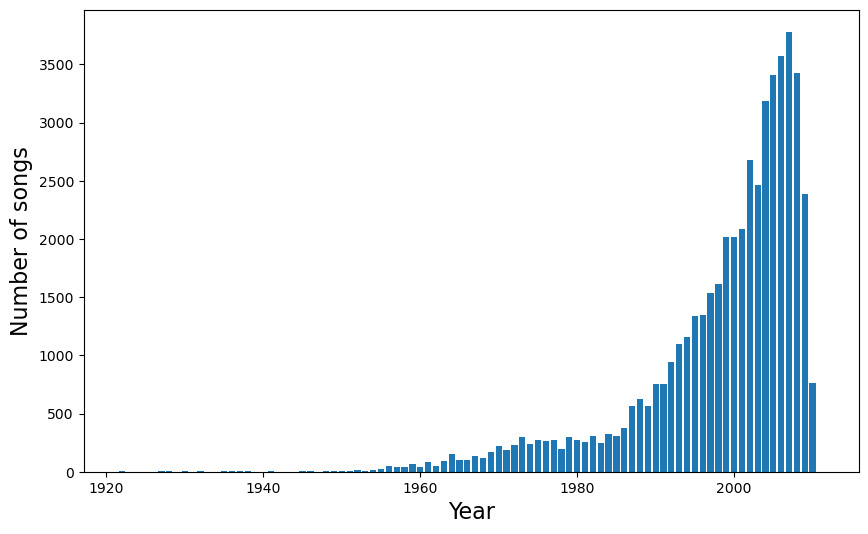
\includegraphics[width=0.95\columnwidth]{images/songs/year_songs.png}
    \caption{Quantity of songs per year in dataset.}
    \label{fig:year_songs}
\end{figure}

\begin{figure}[!htb]
    \centering
    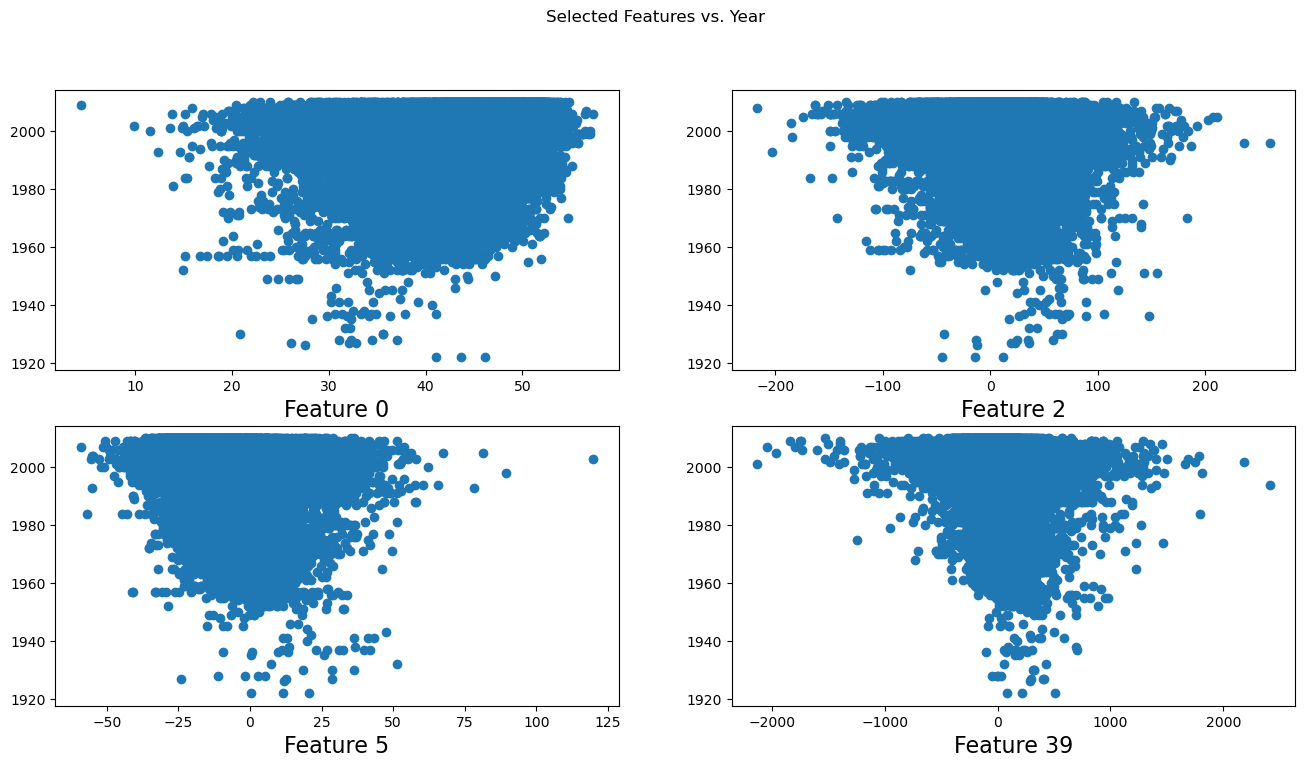
\includegraphics[width=0.95\columnwidth]{images/songs/correlation_best_features.png}
    \caption{Distribution and relation with output of features which correlation with output > 0.12.}
    \label{fig:correlation_best_features}
\end{figure}


\begin{table}
    \centering
    \caption{Cross validation of best models. $ \text{Huber}(\alpha=0.001, \epsilon=1.35)$,
     $ \text{KNN}(n\_neighbors=7, p=2, \text{weights}=\text{'uniform'})$, 
     $ \text{SVR}(C=10.0, \gamma=\text{'scale'}, \text{kernel}=\text{'rbf'})$. 
    Time = time elapsed for all folds. Metrics are the mean over the 5 folds.}
    \label{tab:year_song_cross_validation}
    \begin{tabular}{|l|c|c|c|}
    \toprule
    Model & MAE & MedAE  & Time (s) \\
    \midrule
    Huber & 6.80 & 4.69  & 1.2 \\ 
    SVR & 6.01 & 3.89  & 960.0 \\
    KNN & 6.79 & 4.91  & 10.9 \\
    \bottomrule
    \end{tabular}
\end{table}

\begin{table}
    \centering
    \caption{Test performance of best models. $ \text{Huber}(\alpha=0.001, \epsilon=1.35)$, $ \text{KNN}(n\_neighbors=7, p=2, \text{weights}=\text{'uniform'})$, $ \text{SVR}(C=10.0, \gamma=\text{'scale'}, \text{kernel}=\text{'rbf'})$.}
    \label{tab:test_performance}
    \begin{tabular}{|l|c|c|c|c|c|}
    \toprule
    Model & MAE & MedAE & Fitting T(s) & Predicting T (s) \\
    \midrule
    SVR & 5.91 & 3.89 & 638.19 & 26.90 \\
    Huber & 6.76 & 4.67 & 0.91 & 0.00 \\
    KNN & 6.70 & 5.00 & 0.08 & 0.44 \\
    \bottomrule
    \end{tabular}
\end{table}

\begin{table}
    \centering
    \caption{Screening of classification models with default parameters and PCA=0.95 for the CIFAR-10 dataset.}
    \label{tab:CIFAR_screening}
    \begin{tabular}{|l|c|c|c|c|c|}
    \toprule
    Model & Acc. & F1 & Prec. & Rec. & Fitting T. (s) \\
    \midrule
    LR & 0.37 & 0.37 & 0.37 & 0.37 & 21.98 \\
    SVM & 0.46 & 0.46 & 0.46 & 0.46 & 29.40 \\
    KNN & 0.31 & 0.30 & 0.39 & 0.31 & 28.11 \\
    RF & 0.35 & 0.34 & 0.35 & 0.34 & 40.01 \\
    MLP & 0.39 & 0.39 & 0.39 & 0.39 & 56.40 \\
    \bottomrule
    \end{tabular}
\end{table}

\begin{table}
    \centering
    \caption{Cross-validation performance of classification models wit PCA=0.95.
     $ \text{SVC}(C=1$), $ \text{MLP}(hidden layers =(100,))$.  
     Time = cross-validation time over 5 folds.}
    \label{tab:CIFAR_cross_validation}
    \begin{tabular}{|l|c|c|c|c|c|}
    \toprule
    Model & Acc. & F1 & Prec. & Rec. & T.(s) \\
    \midrule
    SVC & 0.4581 & 0.4561 & 0.4587 & 0.4580 & 87.13 \\
    MLP & 0.3786 & 0.3784 & 0.3795 & 0.3782 & 82.19 \\
    \bottomrule
    \end{tabular}
\end{table}

\begin{table}
    \centering
    \caption{Test performance of SVC models over the CIFAR-10 dataset. $\text{SVC + G = SVC + GIST}$. Both $\text{SVC}(C=1)$. $SVC + G()$ without PCA.}
    \label{tab:test_svc_performance}
    \begin{tabular}{|l|c|c|c|c|c|}
    \toprule
    Model & Acc. & F1 & Prec. & Rec. & Fit. T.(s)\\
    \midrule
    SVC & 0.47 & 0.46 & 0.46 & 0.46 & 43.91\\
    $SVC + G$  & 0.25 & 0.24 & 0.24 & 0.25 & 7.63 \\
    \bottomrule
    \end{tabular}
\end{table}

\begin{figure}[!htb]
    \centering
    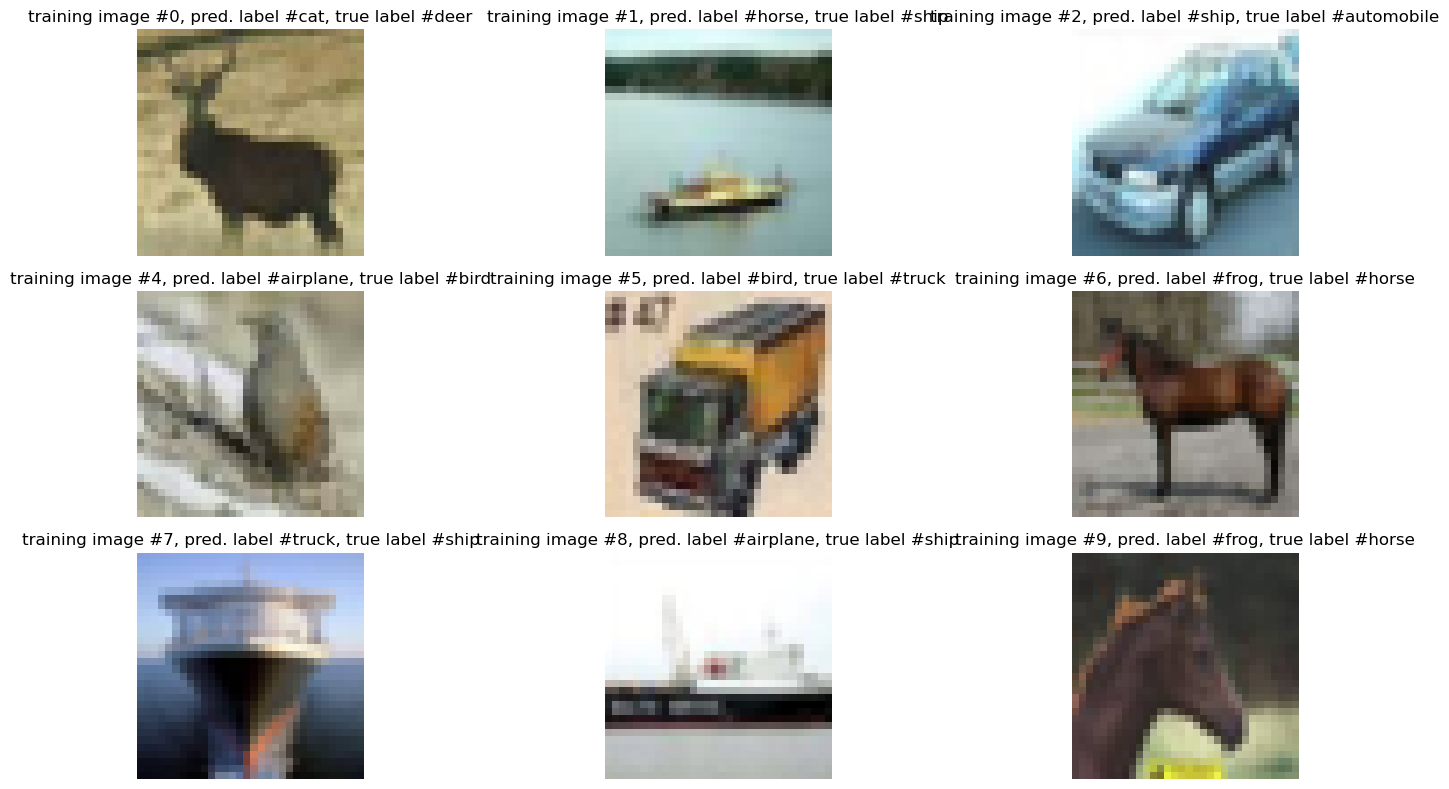
\includegraphics[width=0.95\columnwidth]{images/CIFAR/missclasification_SVM.png}
    \caption{Missclasification of 9 images with $\text{SVC}(C=1)$ and PCA=0.95 over the CIFAR-10 dataset.}
    \label{fig:missclasification_SVM}
\end{figure}

\begin{figure}[!htb]
    \centering
    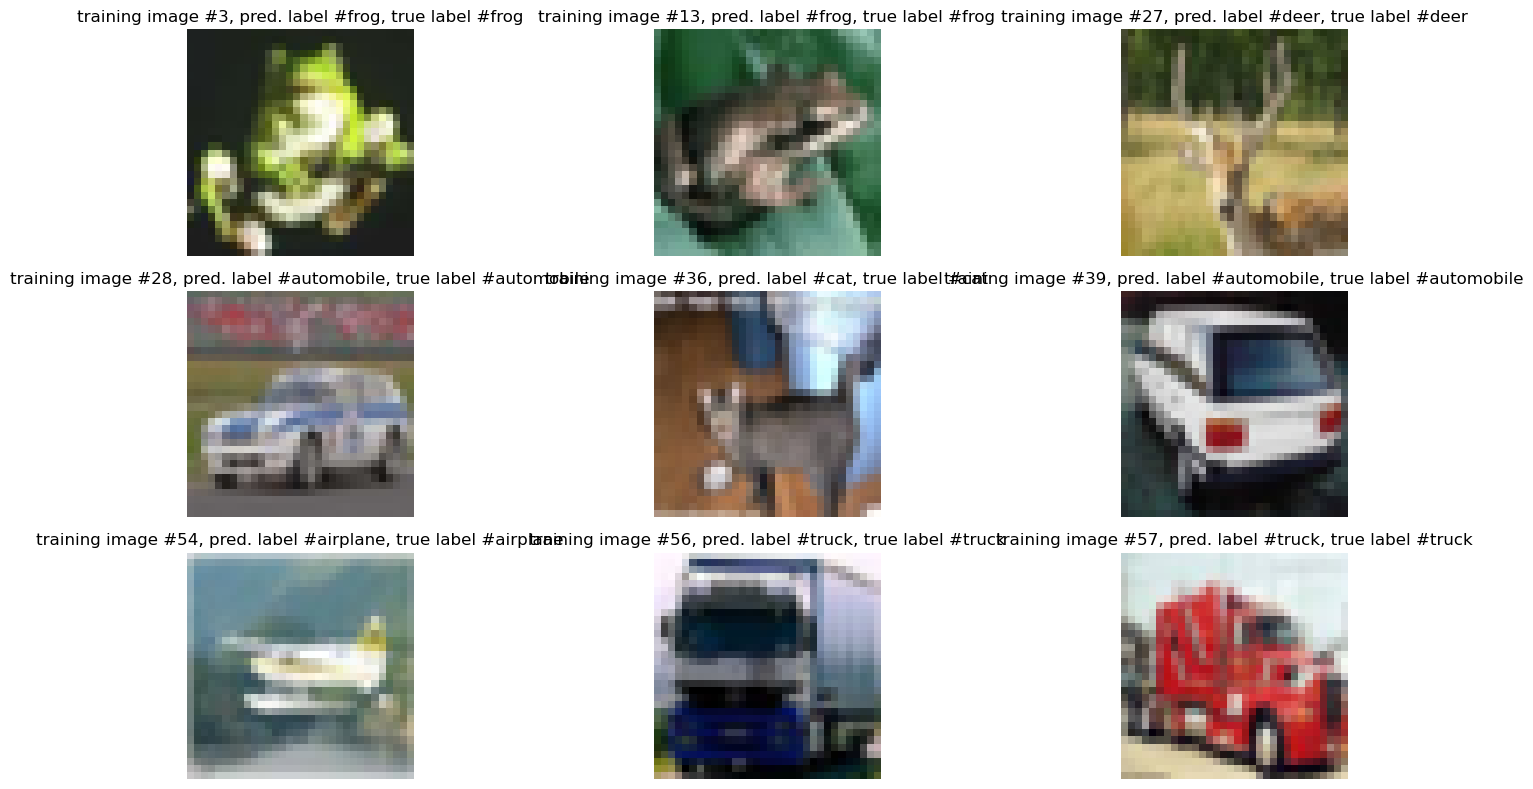
\includegraphics[width=0.95\columnwidth]{images/CIFAR/succes_classification_CIFAR.png}
    \caption{Correct classification of 9 imagaes with $\text{SVC}(C=1)$ and PCA=0.95 over the CIFAR-10 dataset.}
    \label{fig:polynomial_data}
\end{figure}


\end{document}

 
\end{document}


